\documentclass[tikz, border=2pt]{standalone} % border 控制图片边缘留白
\usepackage{amsmath}

\begin{document}
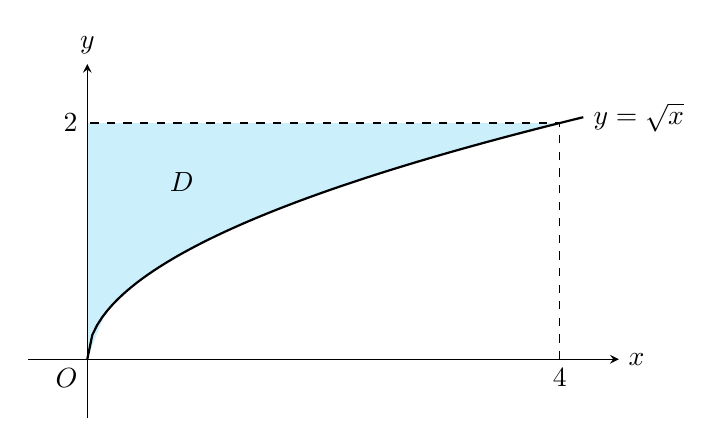
\begin{tikzpicture}[scale=1.5, >=stealth]
    % 填充积分区域 D (此处为 y 轴、y=2 和 y=sqrt(x) 围成的部分)
    \fill[cyan!20] (0,0) -- plot[domain=0:4, smooth] (\x, {sqrt(\x)}) -- (0,2) -- cycle;

    % 画坐标轴
    \draw[->] (-0.5, 0) -- (4.5, 0) node[right] {$x$};
    \draw[->] (0, -0.5) -- (0, 2.5) node[above] {$y$};

    % 画函数曲线 y = sqrt(x)
    \draw[thick, domain=0:4.2, samples=100] plot (\x, {sqrt(\x)}) node[right] {$y=\sqrt{x}$};

    % 画边界辅助线
    \draw[dashed] (4,0) node[below] {$4$} -- (4,2) -- (0,2) node[left] {$2$};

    % 标注区域 D 和原点
    \node at (0.8, 1.5) {$D$};
    \node[below left] at (0,0) {$O$};
\end{tikzpicture}
\end{document}
